\chapter{Redes neuronales}

Este trabajo gira en torno al algoritmo \textit{Word2Vec} \cite{word2vec:1} \cite{word2vec:2}, una técnica de procesamiento
de lenguaje natural, que usa \textit{aprendizaje profundo} para su funcionamiento. El aprendizaje
profundo es una rama del Aprendizaje Máquina, que a su vez está incluido dentro del campo más general
de la Inteligencia Artificial. En general, el objetivo del aprendizaje máquina es estudiar algoritmos
que mejoran a partir de la experiencia. Tom M. Mitchell \cite{mitchell1997} enunció una definición formal
del término:

\begin{definition}
    Se dice que un programa \textit{aprende} de una experiencia \textit{E}, con respecto a un grupo
    de tareas \textit{T} y una medida de rendimiento \textit{P}, si su rendimiento en las tareas de
    \textit{T}, medido por \textit{P}, mejora con la experiencia \textit{E}.
\end{definition}

Estas técnicas suelen estar basadas en el concepto biológico de redes neuronales, las cuales están formadas por neuronas. A lo largo de este capítulo, se va a formalizar este concepto de neurona y se va a definir cómo interactúan entre ellas.

\section{Introducción}

Las redes neuronales suelen ser usadas en objetos que, a priori, no tienen una representación matemática,
como imágenes. El procedimiento habitual es encontrar una representación numérica que permita, de forma
cómoda, operar con esos objetos. Por ejemplo, para representar una imagen en blanco y negro, se puede
tomar un vector $x$, con tantas entradas como píxeles, donde cada entrada es un valor entre 0 y 1,
representando el valor del color en ese píxel. La red neuronal ahora debe tomar ese valor de entrada,
y producir otra representación matemática distinta, que también debe ser interpretada. Por ejemplo,
si se quieren detectar números escritos en la imagen, la representación de salida puede ser un vector
de 10 entradas, donde el valor de cada entrada será igual a 1 si el índice de esa entrada coincide con
el número presente en la imagen.

\begin{figure}[H]
    \centering
    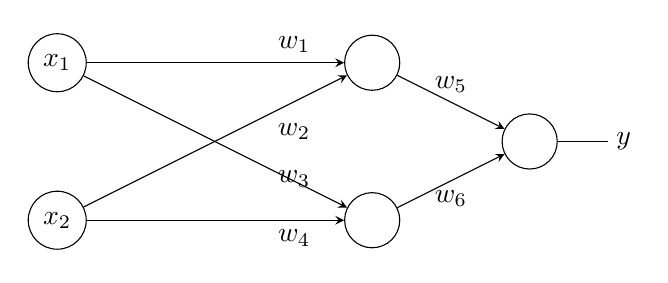
\begin{tikzpicture}[
            roundnode/.style={circle, draw=black, minimum size=7mm},
        ]

        \node[roundnode]   at (1,4)   (input2)  {$x_2$};
        \node[roundnode]   at (1,6)   (input1)  {$x_1$};
        \node[roundnode]   at (5,4)   (hidden2)  {};
        \node[roundnode]   at (5,6)   (hidden1)  {};
        \node[roundnode]   at (7,5)   (output)  {};

        \draw[-stealth] (input1) -- node[above,xshift=1cm]   {$w_1$} (hidden1);
        \draw[-stealth] (input2) -- node[above,xshift=1cm, yshift=-0.1cm]   {$w_2$} (hidden1);
        \draw[-stealth] (input1) -- node[above, xshift=1cm, yshift=-0.7cm] {$w_3$} (hidden2);
        \draw[-stealth] (input2) -- node[below, xshift=1cm]   {$w_4$} (hidden2);

        \draw[-stealth] (hidden1) -- node[above]   {$w_5$} (output);
        \draw[-stealth] (hidden2) -- node[below]   {$w_6$} (output);

        \draw[] (output) -- node[right, xshift=0.3cm] {$y$} (8,5);

    \end{tikzpicture}
    \caption{Ejemplo de red neuronal con una capa escondida}
    \label{redneuronal:1}
\end{figure}

\subsection{Conceptos iniciales}

Para a partir de un vector de entrada $x\in\mathbb{R}^n$, producir un vector de salida $v\in\mathbb{R}^m$,
con el resultado que se quiere, será necesario realizar ciertas operaciones entra cada una de las capas
de la red neuronal, como se muestra en la Figura \ref{redneuronal:1}. Cada una de estas operaciones, activará
algunas neuronas en cada capa, produciendo al final el vector deseado. Una neurona no es más ni menos
que un escalar, entre 0 y 1 normalmente, cuyo valor es calculado usando el valor de las neuronas de la
capa anterior (o del input, si es la segunda capa) junto con el valor de los pesos $w_i$:

\[
    a^{(n+1)} = a^{(n)}_1w^{(n)}_1+a^{(n)}_2w^{(n)}_2+\cdots+a^{(n)}_nw^{(n)}_n=\sum_{i=1}^na^{(n)}_iw^{(n)}_i\in\mathbb{R}
\]

Los pesos no son más que números arbitrarios, que son actualizados en cada fase de aprendizaje \cite{rumelhart1986learning}.
Es trivial comprobar que $a^{(n+1)}$ es un número real, de cualquier valor. Esto es problemático porque
lo que se quiere ahora es saber cuando una neurona está \textit{activa}. Para ello, se puede usar lo
que se denomina una \textit{función de activación}, que no es ni más ni menos que una función  que transforma
la recta real en el intervalo $[0,1]$. Intuitivamente, el valor que devuelve la función de activación dice
cómo de positivo es el valor de esa neurona. Hay muchas elecciones posibles de función de activación, a continuación
se proponen algunas.

\subsubsection{Sigmoide}

La función sigmoide está definida como:
\begin{align*}
    \sigma \colon & \mathbb{R} \longrightarrow ]0,1[             \\
    \quad         & x \longmapsto \sigma(x) = \frac{1}{1+e^{-x}}
\end{align*}

Esta función es una de las más usada como función de activación. Entre sus principales ventajas está que es diferenciable, monótona y regular. Además, tiene dos características que serán usadas posteriormente:
\begin{equation} \label{sigmoid:1}
    \sigma(-x)=1-\sigma(x)
\end{equation}
\begin{equation} \label{sigmoid:2}
    \frac{d\sigma(x)}{dx}=\sigma(x)\sigma(-x)
\end{equation}

\begin{figure}[H]
    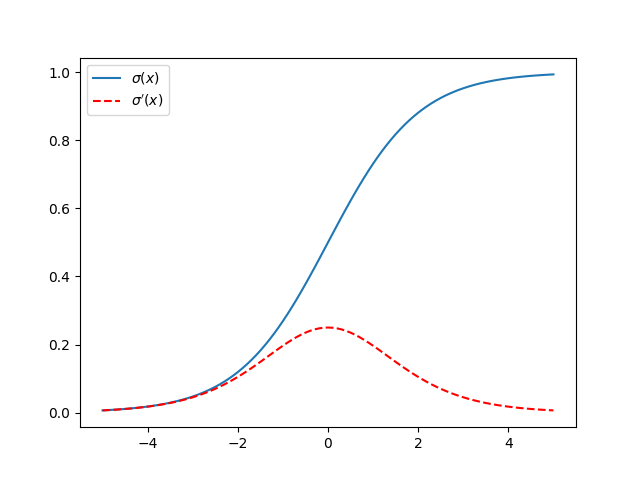
\includegraphics[width=7cm]{sigmoid.png}
    \centering
\end{figure}

El principal problema de esta función se denomina \textit{vanishing problem} \cite{hochreiter1991untersuchungen}.
Cuando se avance un poco más en los fundamentos de las redes neuronales, se volverá a este problema.

\subsubsection{Tangente Hiperbólica}

La función tangente hiperbólica está definida como:
\begin{align*}
    f \colon & \mathbb{R} \longrightarrow ]0,1[                       \\
    \quad    & x \longmapsto f(x) = \frac{e^{x}-e^{-x}}{e^{x}+e^{-x}}
\end{align*}

En el gráfico de esta función, se puede apreciar que su derivada es más pronunciada que la de la función sigmoide. Esto permite a la red neuronal aprender de forma más rápida, haciendo el aprendizaje más eficiente.

\begin{figure}[H]
    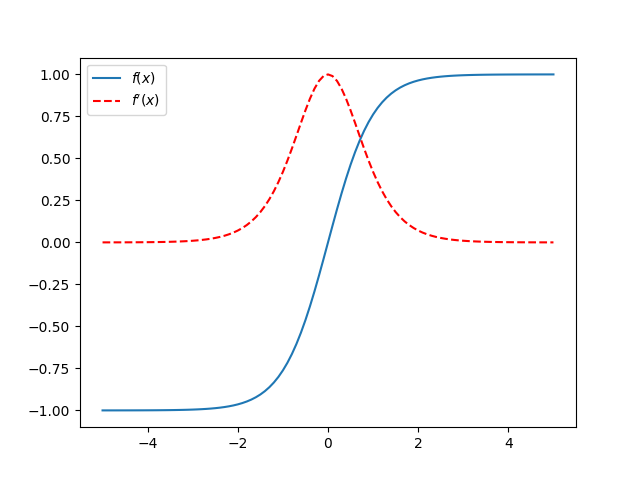
\includegraphics[width=7cm]{tanh.png}
    \centering
\end{figure}

\subsubsection{Unidad Linear Rectificada (ReLU)}

La función ReLU está definida por:
\begin{align*}
    f \colon & \mathbb{R} \longrightarrow ]0,1[ \\
    \quad    & x \longmapsto f(x) = \max(0,x)
\end{align*}

Evidentemente, está función es mucho más eficiente, computacionalmente hablando, que las dos primeras alternativas. Sin embargo, presenta un gran problema: cuando los valores de entrada se aproximan o son inferiores a 0, la red no puede efectuar propagación hacia atrás, por lo que no puede aprender.

\begin{figure}[H]
    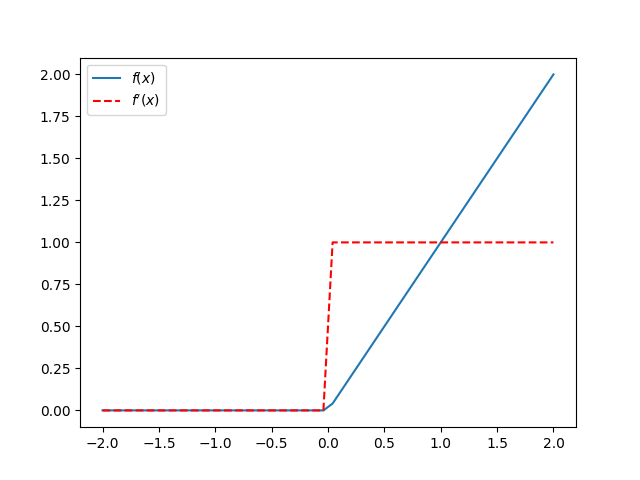
\includegraphics[width=7cm]{relu.png}
    \centering
\end{figure}


Por lo tanto, después de este razonamiento, el valor de cada neurona se calculará siguiendo la expresión:

\begin{equation}
    \label{eqn:1}
    a^{(n+1)}_j = f\left( b^{(n)}_j + \sum_{i=1}^n a^{(n)}_i w^{(n)}_i \right) \in [0,1]
\end{equation}

donde $b^{(n)}$ es otro valor arbitrario que va siendo actualizado para modificar el valor de salida de la
función de activación $f$.

\subsection{Notación}

Las redes neuronales suelen ser más complejas que la expuesta en la Figura \ref{redneuronal:1}. Normalmente,
se tienen muchos más inputs, pesos y capas escondidas. Por esa razón, una notación matricial para describir
las operaciones que se van a realizar es bastante adecuada. Como se verá en el siguiente capítulo, nuestra
red neuronal de interés solo tiene una capa escondida, así que se adaptará la notación a ese hecho:

\begin{itemize}
    \item Los subíndices $k$, $i$ y $j$ serán usados para denotar los valores de entrada, los valores de la
          capa escondido y los valores de salida, respectivamente.
    \item $x_1, \ldots x_K$ es el vector con los valores de entrada.
    \item $h_1, \ldots h_N$ es el vector con los valores de la capa escondida.
    \item $y_1, \ldots y_M$ es el vector con los valores de salida.
    \item $W = (w_{ki})$ es una matriz de dimensiones $n\times m$, donde $n$ es la dimensión
          del vector de entrada, $m$ la dimensión del vector de valores de la capa escondida y $w_{ki}$ es el peso de la conexión de la
          neurona $x_k$ con la neurona $h_i$.
    \item $W' = (w_{ij}')$ es una matriz de dimensiones $m\times q$, donde $m$ es la dimensión
          del vector de valores de la capa escondida, $q$ es la dimensión del vector de salida y $w_{ki}'$
          es el peso de la conexión de la neurona $h_i$ con la neurona $y_j$.
\end{itemize}

\begin{figure}[H]
    \centering
    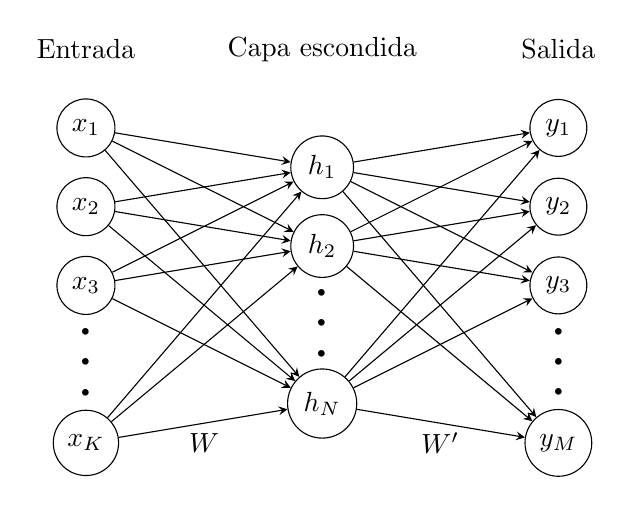
\begin{tikzpicture}[
            roundnode/.style={circle, draw=black, minimum size=3mm},
        ]

        \node[] at (0,5) {Entrada};
        \node[] at (3,5) {Capa escondida};
        \node[] at (6,5) {Salida};

        \node[roundnode]   at (0,0)   (inputK)  {$x_K$};
        \node[roundnode]   at (0,2)   (input3)  {$x_3$};
        \node[roundnode]   at (0,3)   (input2)  {$x_2$};
        \node[roundnode]   at (0,4)   (input1)  {$x_1$};

        \path (input3) -- (inputK) node [black, font=\Huge, midway, sloped] {$\dots$};

        \node[roundnode]   at (3,0.5)   (hiddenN)  {$h_N$};
        \node[roundnode]   at (3,2.5)   (hidden2)  {$h_2$};
        \node[roundnode]   at (3,3.5)   (hidden1)  {$h_1$};

        \path (hidden2) -- (hiddenN) node [black, font=\Huge, midway, sloped] {$\dots$};

        \node[roundnode]   at (6,0)   (outputM)  {$y_M$};
        \node[roundnode]   at (6,2)   (output3)  {$y_3$};
        \node[roundnode]   at (6,3)   (output2)  {$y_2$};
        \node[roundnode]   at (6,4)   (output1)  {$y_1$};

        \path (output3) -- (outputM) node [black, font=\Huge, midway, sloped] {$\dots$};

        \draw[-stealth] (input1) -- (hidden1);
        \draw[-stealth] (input2) -- (hidden1);
        \draw[-stealth] (input3) -- (hidden1);
        \draw[-stealth] (inputK) -- (hidden1);

        \draw[-stealth] (input1) -- (hidden2);
        \draw[-stealth] (input2) -- (hidden2);
        \draw[-stealth] (input3) -- (hidden2);
        \draw[-stealth] (inputK) -- (hidden2);

        \draw[-stealth] (input1) -- (hiddenN);
        \draw[-stealth] (input2) -- (hiddenN);
        \draw[-stealth] (input3) -- (hiddenN);
        \draw[-stealth] (inputK) -- (hiddenN);

        \draw[-stealth] (hidden1) -- (output1);
        \draw[-stealth] (hidden1) -- (output2);
        \draw[-stealth] (hidden1) -- (output3);
        \draw[-stealth] (hidden1) -- (outputM);

        \draw[-stealth] (hidden2) -- (output1);
        \draw[-stealth] (hidden2) -- (output2);
        \draw[-stealth] (hidden2) -- (output3);
        \draw[-stealth] (hidden2) -- (outputM);

        \draw[-stealth] (hiddenN) -- (output1);
        \draw[-stealth] (hiddenN) -- (output2);
        \draw[-stealth] (hiddenN) -- (output3);
        \draw[-stealth] (hiddenN) -- (outputM);


        \node[] at (1.5,0) {$W$};
        \node[] at (4.5,0) {$W'$};

    \end{tikzpicture}
    \caption{Red neuronal con una capa escondida}
    \label{redneuronal:2}
\end{figure}

Con esta nueva notación, la expresión \ref{eqn:1}, puede escribirse como:

\begin{equation}
    \label{eqn:2}
    h_i = f(u_i) = f\left(\sum_{k=1}^K w_{ki} x_k\right), \;\;\;\;\;
    y_j = f(u_i') = f\left(\sum_{i=1}^N w_{ij}' h_i\right)
\end{equation}

\section{Descenso de gradiente}

Una vez se han definido los elementos de una red neuronal, es necesario definir cómo esa red neuronal
va a \textit{aprender}. Para ello, primero es necesario encontrar una forma de medir cómo de correcto
es el resultado de nuestra red neuronal, es decir, se va a definir una función que mida el error obtenido.
Dado que los vectores de salida son numéricos, se puede tomar simplemente la suma de la diferencia al
cuadrado entre el resultado de la red $y = (y_1, \ldots, y_M)$ y la salida esperada $t = (t_1, \ldots, t_M)$:

\begin{equation}
    \label{eqn:3}
    E(x, t, W, W') = \frac{1}{2}\sum_{j=1}^M(y_j-t_j)^2
\end{equation}

A partir de las ecuaciones \ref{eqn:2}, la dependencia de $x$, $W$ y $W'$ en la definición del error se
El objetivo a lo largo de esta sección va a ser minimizar esa función multidimensional.
ve de forma inmediata.

El algoritmo que se va a usar se denomina \textit{descenso de gradiente} \cite{lemarechal2012cauchy}.
Su nombre proviene del hecho
que el gradiente de una función multidimensional da como resultado la dirección más \textit{empinada},
o también se puede decir que el gradiente, siempre va \textit{cuesta arriba}. Sea $f \colon \mathbb{R}^n \longrightarrow \mathbb{R}$
una función multidimensional y $\nabla f$ su gradiente, es trivial deducir que entonces $-\nabla f$
siempre va \textit{cuesta abajo}. Este hecho puede ser explotado para encontrar mínimos, en principio locales,
de $f$, usando la expresión:


\begin{equation}
    \label{eqn:gradient_descent}
    x'=x-\epsilon\nabla f(x)
\end{equation}

donde $\epsilon$ es un escalar positivo, pequeño y arbitrario, denominado \textit{ratio de aprendizaje}.
Para la elección de $\epsilon$, se pueden tomar
varias opciones:

\section{Back-propagation}

En el caso particular de redes neuronales, este algoritmo se usará para actualizar el valor de los pesos
de forma que el error definiedo en \ref{eqn:3}, sea mínimo. A este algoritmo, se le conoce como
\textit{back-propagation} \cite{rumelhart1986learning}. Adaptando la expresión del descenso de gradiente al caso más sencillo, se obtiene:

\begin{equation}
    \label{eqn:gradient_descent_nn}
    w^{(nueva)}=w^{(vieja)}-\epsilon (y-t)y(1-y)x
\end{equation}

donde $y$ es el valor de salida, $t$ el valor que se quiere y $x$ el valor de entrada. Para obtener esa
expresión en el caso de una red neuronal con una capa escondida, son necesarios algunos pasos adicionales.
Primero, es necesario derivar el error con respecto al valor de entrada:
\[
    \frac{\partial E}{\partial y_j} = y_j - t_j
\]
Una vez ese valor es conocido, se puede calcular la derivada respecto $u_j'$:
\[
    \frac{\partial E}{\partial u_j'} =     \frac{\partial E}{\partial y_j}     \frac{\partial y_j}{\partial u_j'}=
    (y_j-t_j)y_j(1-y_j) := EI_j'
\]
A este valor se le va a denotar $EI_j'$ porque es usado en los siguientes cálculos. Siguiendo ahora con $w_{ij}'$:
\[
    \frac{\partial E}{\partial w_{ij}'} =     \frac{\partial E}{\partial u_j'}     \frac{\partial u_j'}{\partial w_{ij}'} =
    EI_j' h_i
\]
Por lo tanto, aplicando el método de descenso de gradiente, se han obtenido las ecuaciones para actualizar los pesos
entre la capa escondida y la capa de salida:
\[
    w_{ij}'^{(nuevo)} = w_{ij}'^{(viejo)} - \epsilon \frac{\partial E}{\partial w_{ij}'} =
    w_{ij}'^{(viejo)}-\epsilon EI_j' h_i
\]

A continuación se va a realizar el paso que le da nombre a este algoritmo. Repitiendo el cálculo anterior
pero para la capa de entrada y la escondida, es decir, considerando $h_i$, $u_i$ y $w_{ki}$, es posible
actualizar su matriz de pesos teniendo en cuenta la optimización obtenida en la capa anterior. Por lo tanto,
derivando respecto de $h_i$:
\[
    \frac{\partial E}{\partial h_i} = \sum_{j=1}^M\frac{\partial E}{\partial u_j'} \frac{\partial u_j'}{\partial h_i} =
    \sum_{j=1}^M EI_j' w_{ij}'
\]
Continuando con $u_i$, una vez más se denota el valor obtenido por su importancia en cálculos posteriores:
\[
    \frac{\partial E}{\partial u_i} =     \frac{\partial E}{\partial h_i}     \frac{\partial h_i}{\partial u_i} =
    \sum_{j=1}^M  EU_j' w_{ij}' h_i (1-h_i) := EI_i
\]
Y por último:
\[
    \frac{\partial E}{\partial w_{ki}} = \frac{\partial E}{\partial u_i} \frac{\partial u_i}{\partial w_{ki}} =
    EI_i x_k
\]
Obteniendo, finalmente, la ecuación para actualizar los pesos entre la capa de entrada y la escondida:
\[
    w_{ki}^{(nuevo)} = w_{ki}^{(viejo)} - \epsilon \frac{\partial E}{\partial w_{ki}} =
    w_{ij}^{(viejo)}-\epsilon EI_i x_k
\]